\section{实现与测试}
\subsection{总体实现}
最终完成的部分有一个网页程序和一个本地程序,内容是同样的一个网页。均可
以通过按照需求描述的各种方法录入文法,并且可以将文法保存起来,而无需多
次重复输入文法。当前的实现中,缺少对词法分析的动画的支持,而实现了语法
分析动画的支持。
\subsection{使用}
用户首先需要下载这个程序,直接打开对应的网页或者本地程序,即可以使用,
另一种方式是将网页部署到服务器上面,然后打开对应的链接开始使用这个程序。

用户首先需要输入文法,通过文件上传拖拽或者是直接输入都可以。之后就可以
按照流程进行,分别是左递归消除、提取公因式、然后生成分析表,最后可以拿
着分析表分析用户输入的字符串。

在这些过程中,用户都可以通过控制栏来查看动画演示、算法步骤演示,在演示
过程中不能再更改相关的数据,而用户可以进行前进后退,而不仅仅只是往前看
动画演示。在界面的相应位置,用户可以看到当前的状态显示是如何的。用户还
可以将演示结果保存下来或者打印出来,生成相应的报告。

用户还可以将状态保存起来,下次打开程序的时候(网页或者本地程序)都可以
恢复到特定的状态,而无需重新调整到对应的状态。
\begin{figure}[!htb]
	\centering
	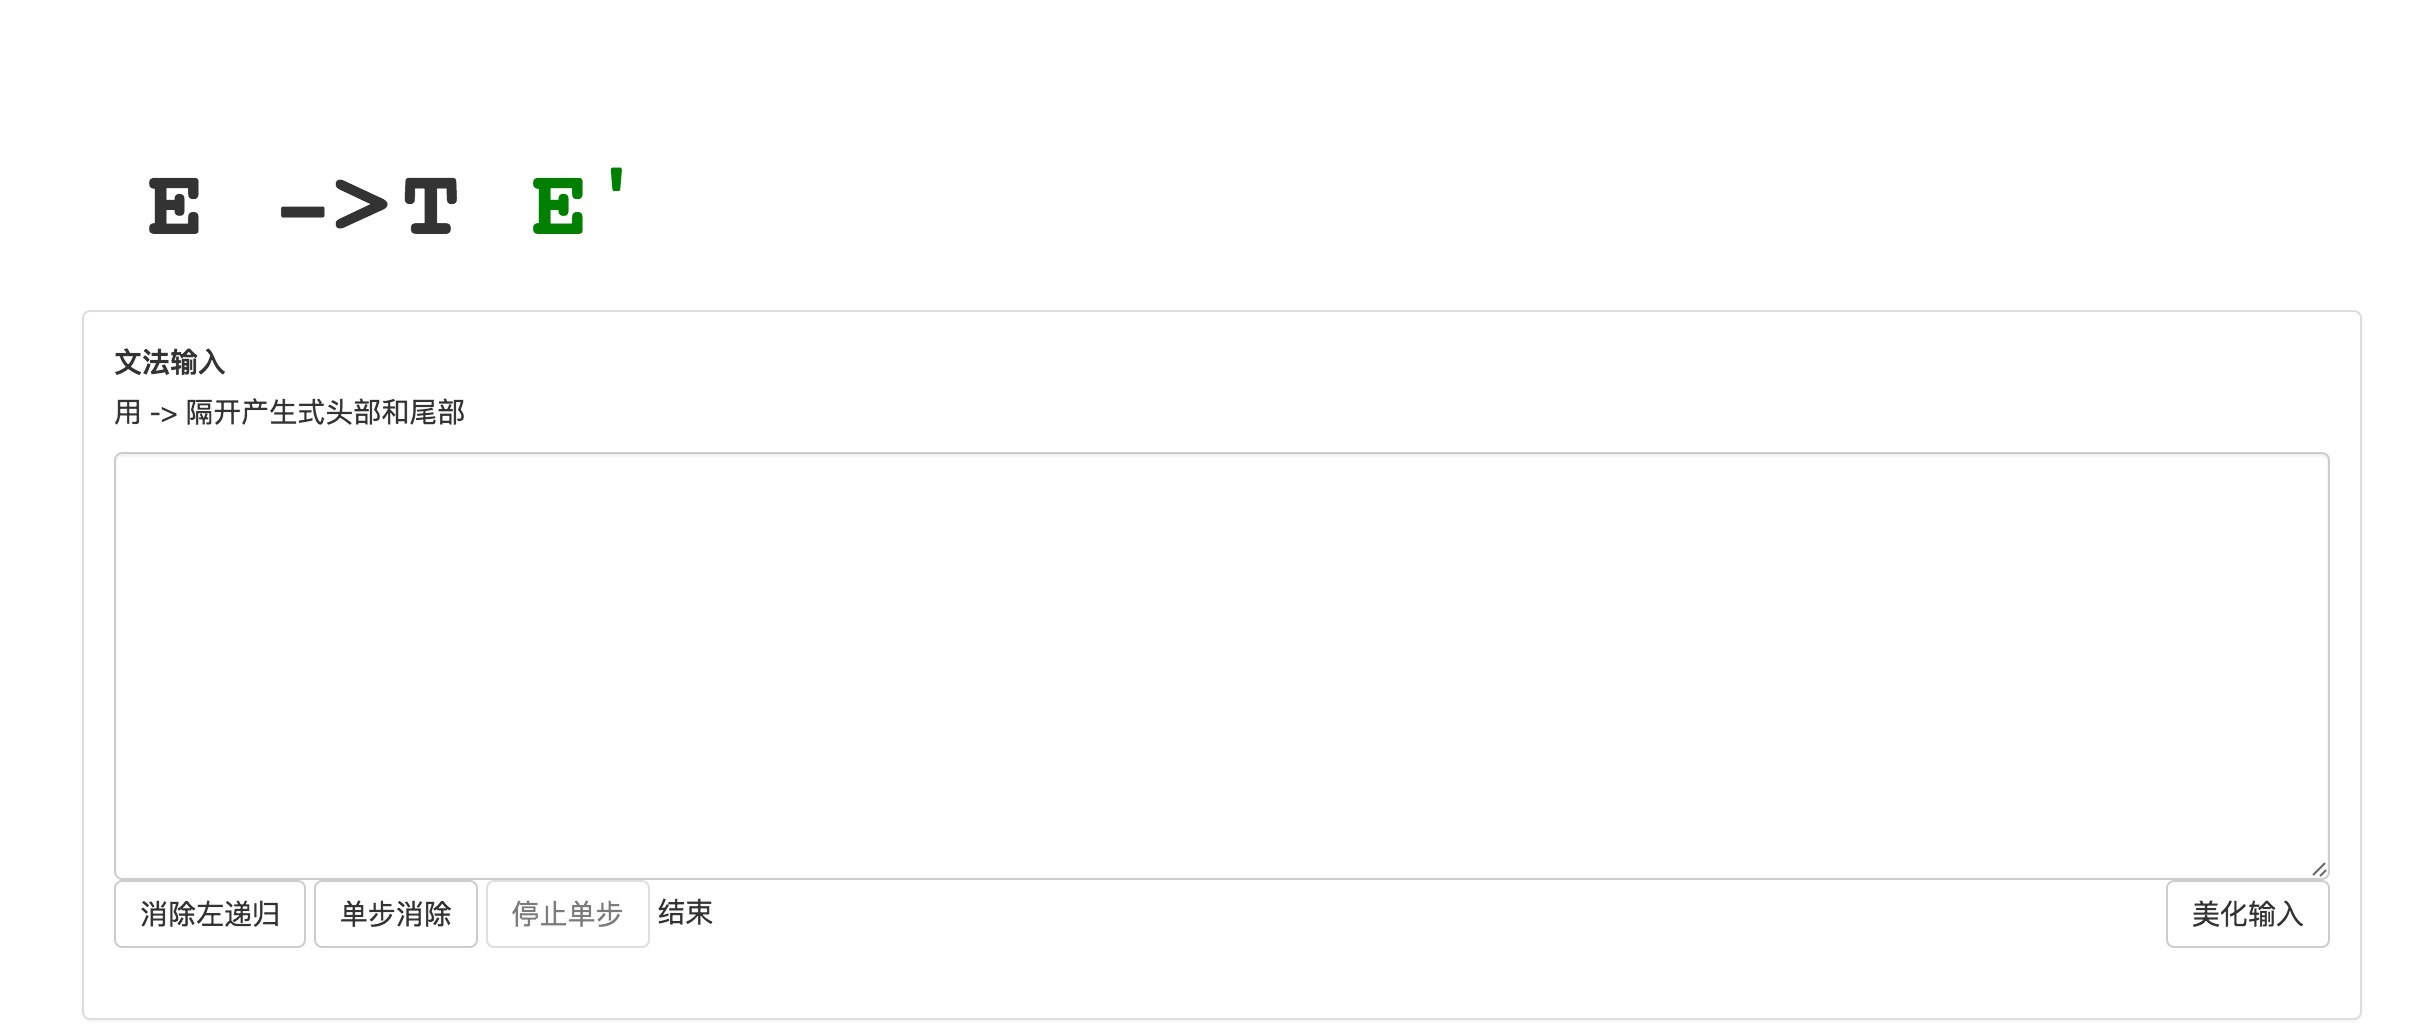
\includegraphics[width=1\linewidth]{img/grammarinput2.jpg}
	\caption{输入文法的初版}
	\label{fig:grammarinput2.jpg}
\end{figure}

\begin{figure}[!htb]
	\centering
	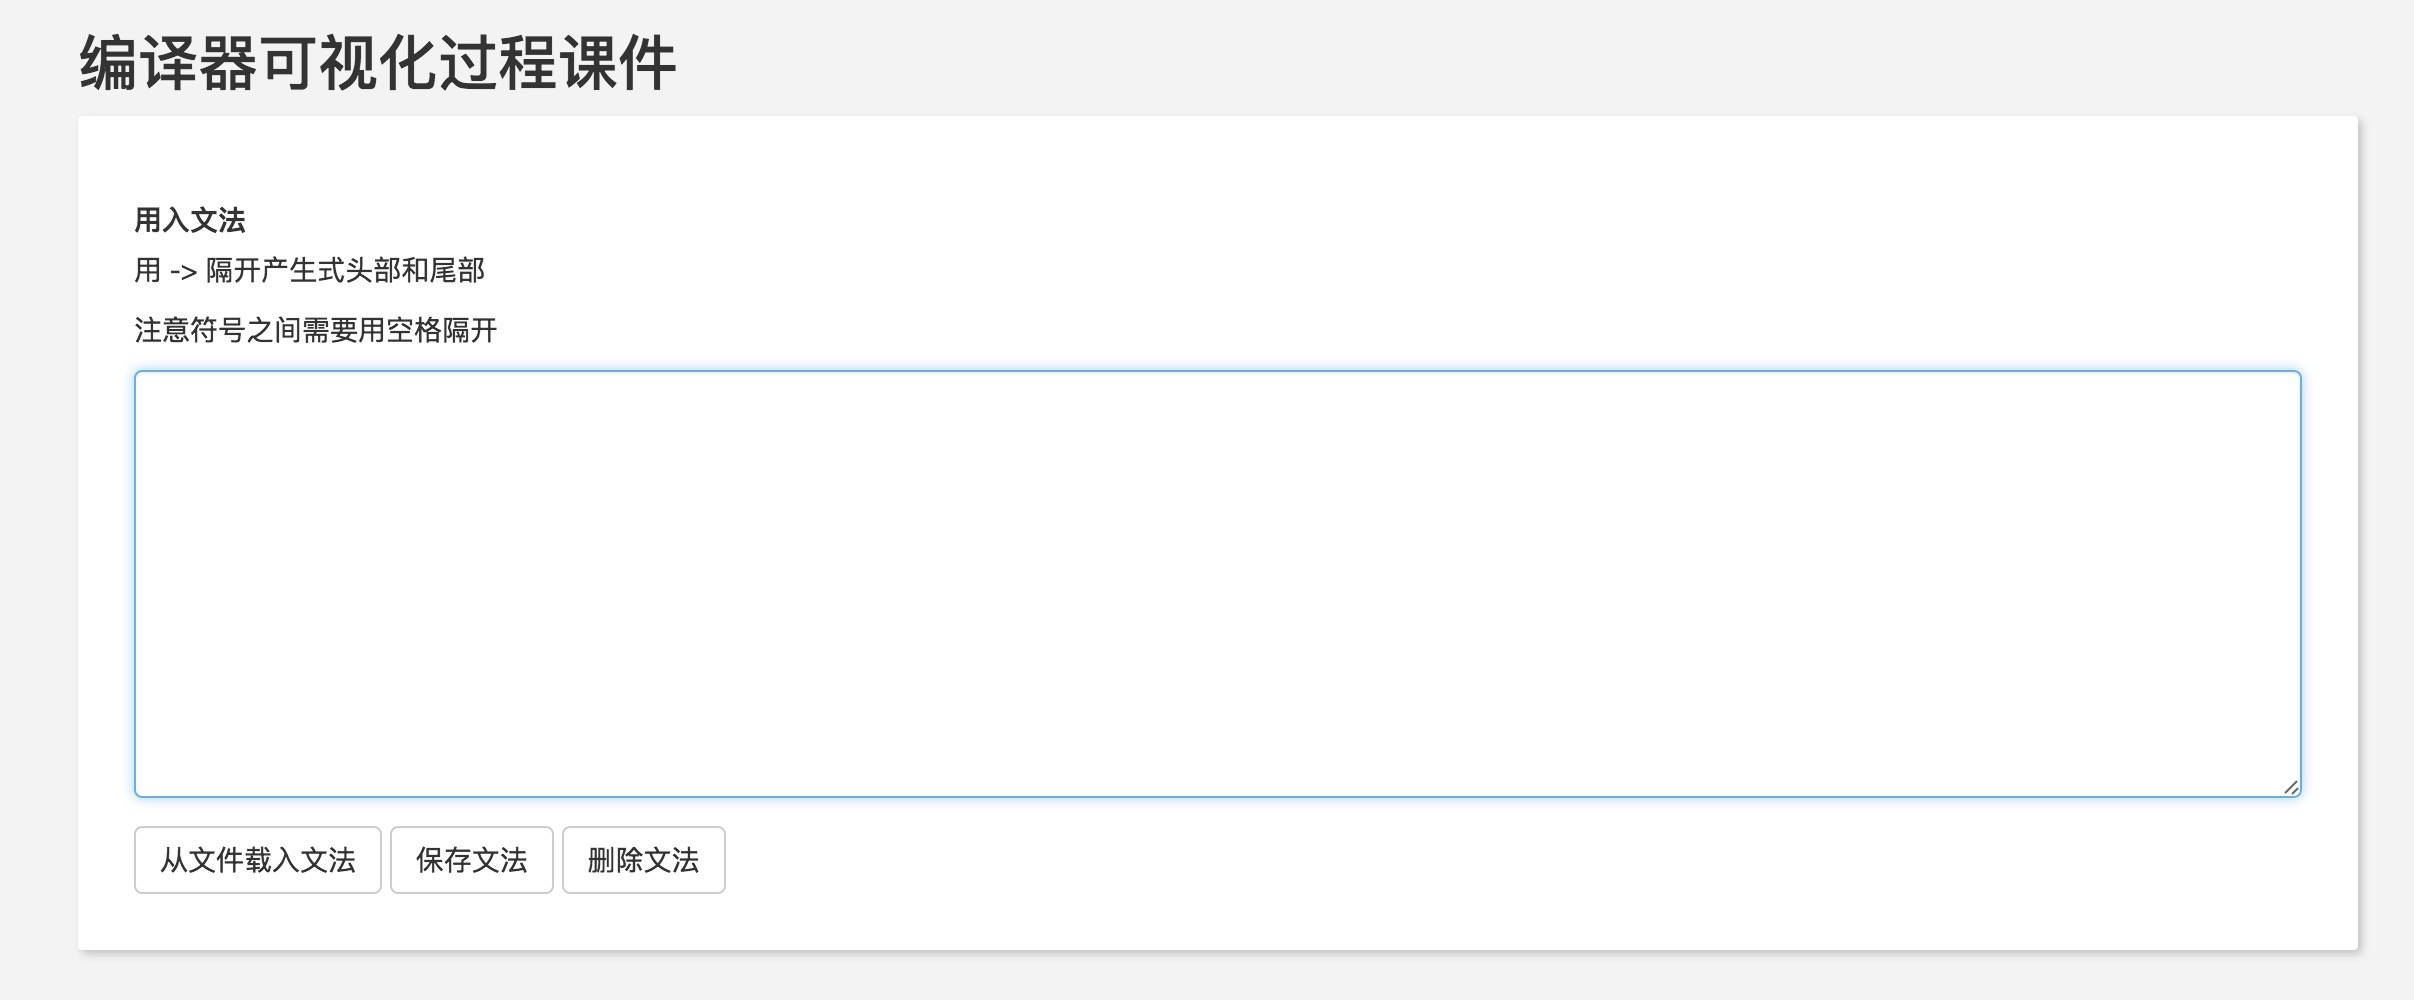
\includegraphics[width=1\linewidth]{img/grammarinput3.jpg}
	\caption{输入文法,可以通过多种方式载入文法}
	\label{fig:grammarinput3.jpg}
\end{figure}

\begin{figure}[!htb]
	\centering
	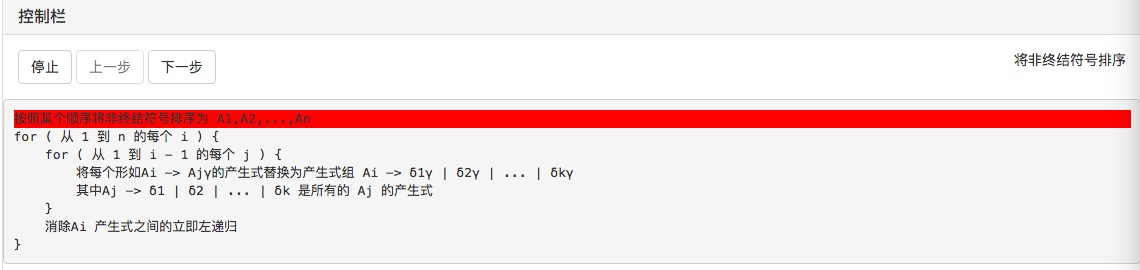
\includegraphics[width=1\linewidth]{img/leftrecursive2.png}
	\caption{左递归消除的算法步骤演示部分}
	\label{fig:leftrecursive2.png}
\end{figure}

\begin{figure}[!htb]
	\centering
	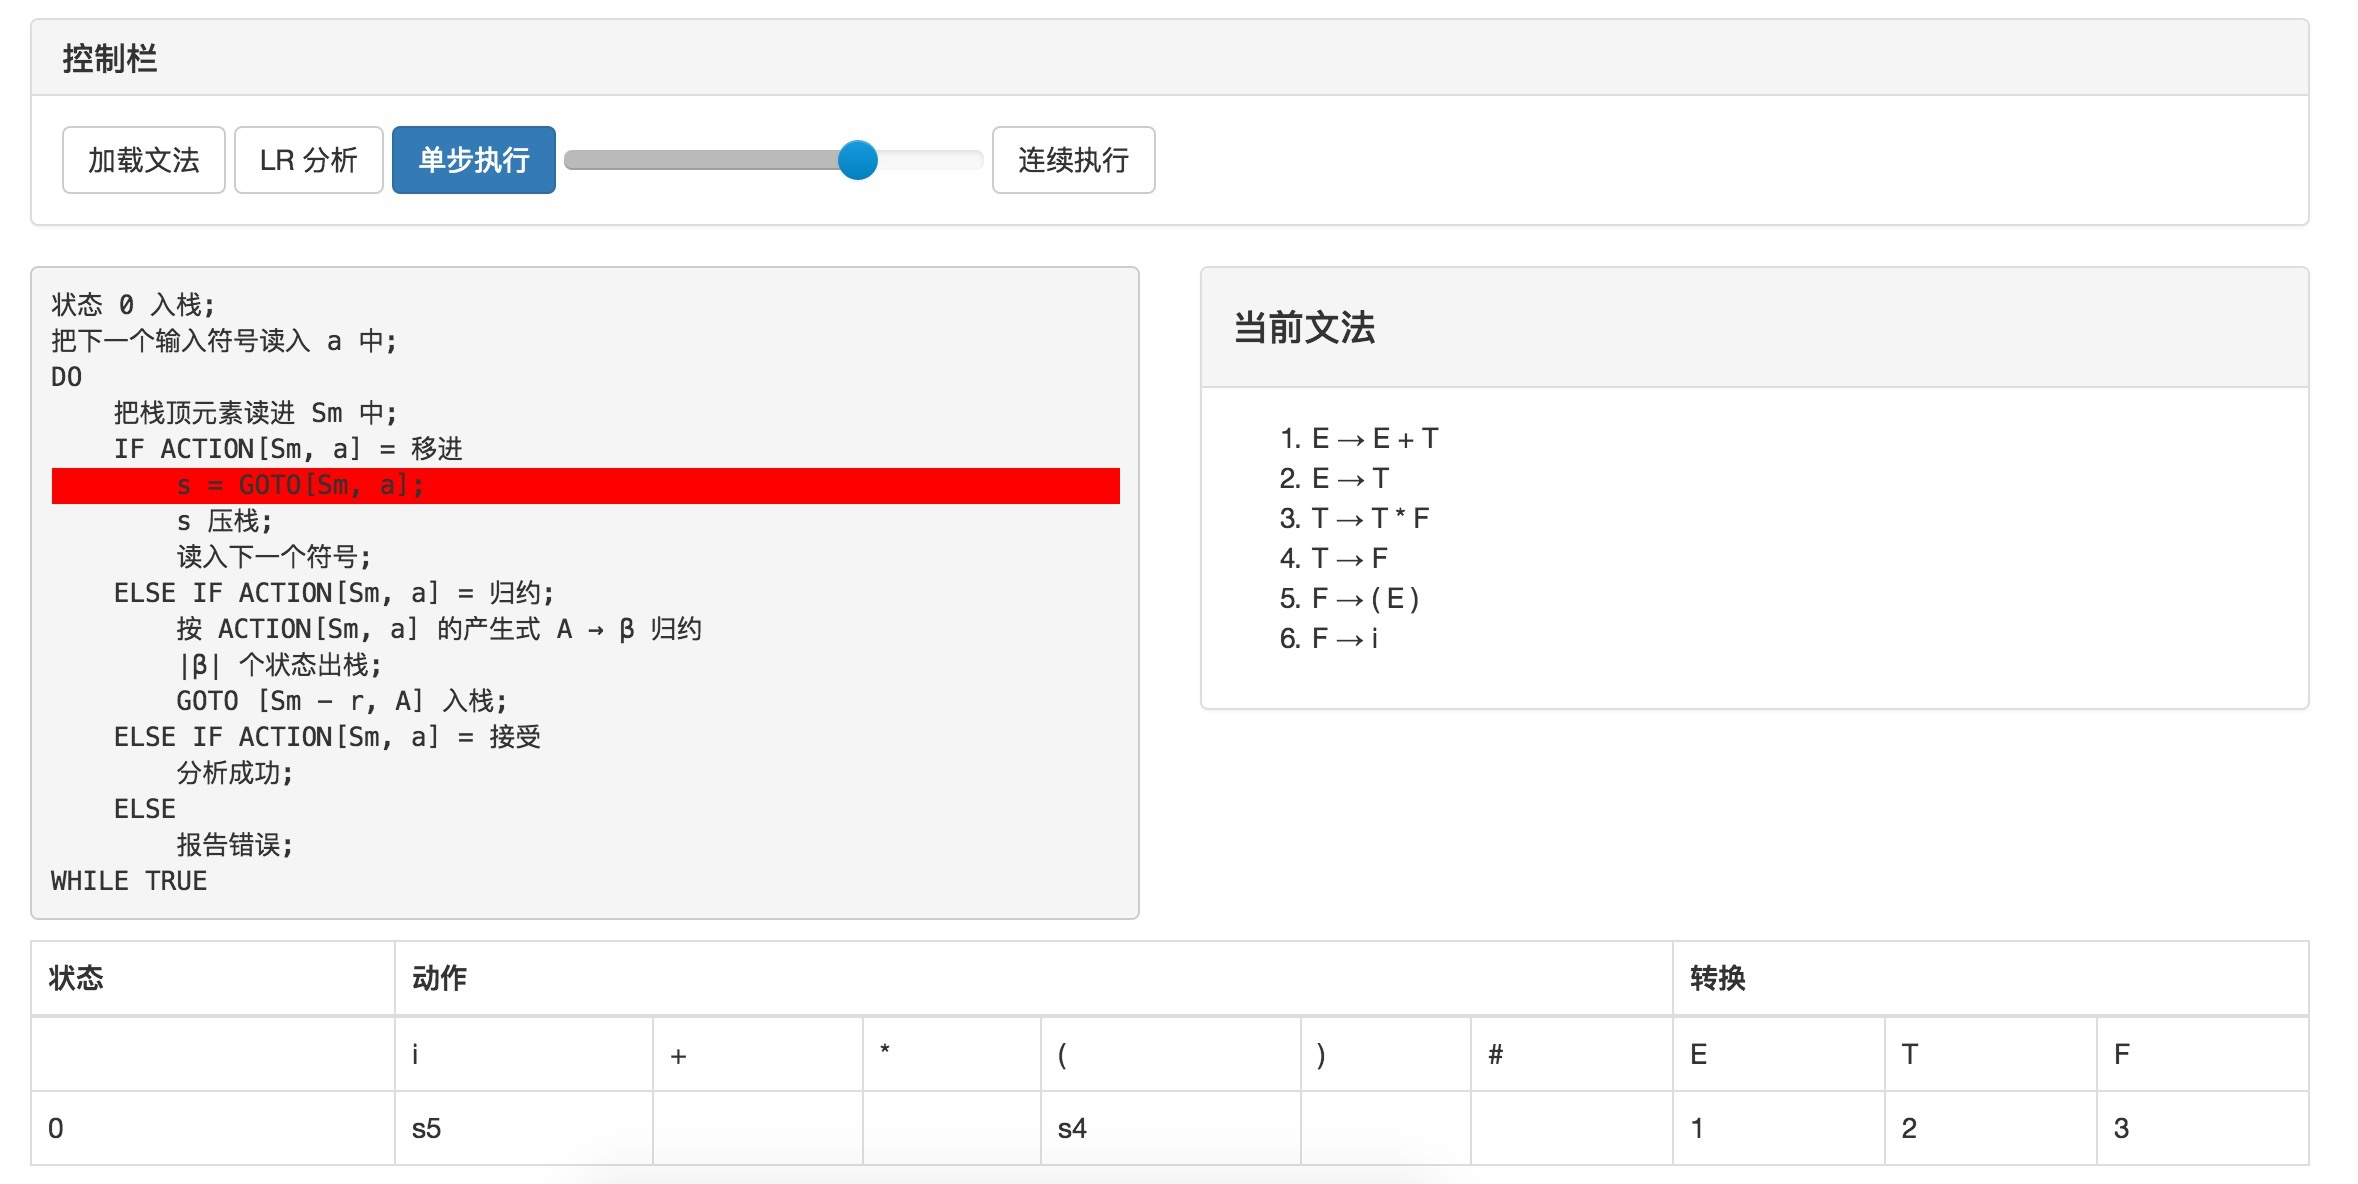
\includegraphics[width=1\linewidth]{img/tableanalyze.jpg}
	\caption{预测分析表的算法步骤演示部分}
	\label{fig:tableanalyze.jpg}
\end{figure}

\begin{figure}[!htb]
	\centering
	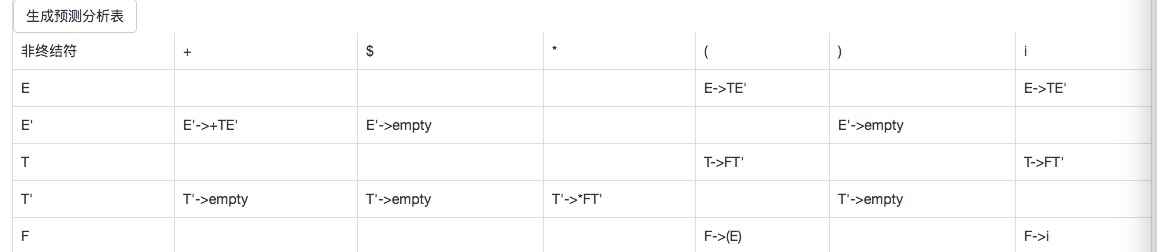
\includegraphics[width=1\linewidth]{img/table.png}
	\caption{预测分析表}
	\label{fig:table.png}
\end{figure}

\begin{figure}[!htb]
	\centering
	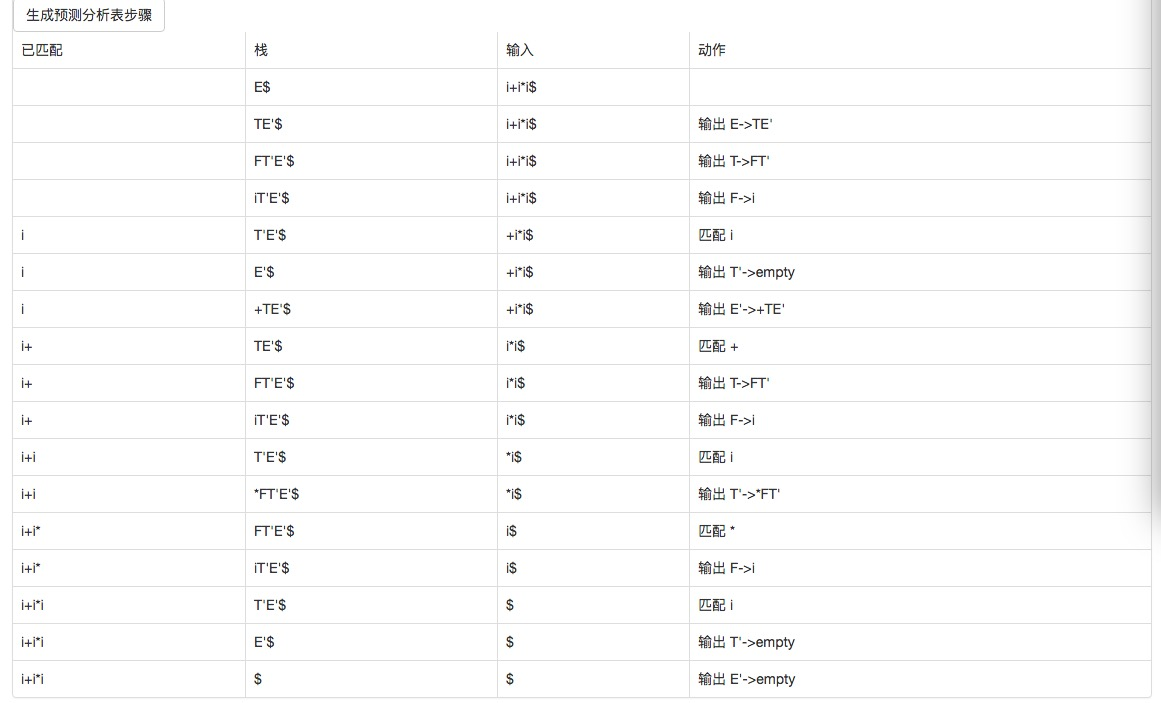
\includegraphics[width=1\linewidth]{img/tablegenerator.png}
	\caption{预测分析表执行步骤演示部分}
	\label{fig:tablegenerator.png}
\end{figure}

\subsection{界面测试}
界面主要是通过手工进行测试,相关的工具也有很多,但是考虑到系统的复杂性,
到目前的阶段还不需要引入专门的界面测试。而手工测试,主要集中在一下几方
面,分别是交互性测试,用来判断交互是否符合逻辑,是否存在错误的交互方法,
是否有交互的缺陷,兼容性测试,主要是针对不同浏览器的显示情况进行测试,
这部分测试我们不是很看重,能在大多数主流浏览器上能够运行即可,界面元素
和预想的偏差都不用在意,因为我们主要的目标平台是固定的浏览器,特别是,
我们可以要求用户安装特定的浏览器。还有其他的界面测试,比如界面的稳定性
测试,指的是在程序运行的时候,界面会不会卡顿,会不会出现一些不稳定的抖
动现象,会不会有一些不良的图像噪音,动画过程是否流畅等等。
\subsection{单元测试}
对于单元测试,我们将程序重构成由一个一个类组成的模块的时候,单元测试就
已经变得容易起来了。特别是,我们之后还严格控制了,底层逻辑的部分是不会
直接访问界面的元素,保证所有非界面相关的类都不会直接和界面联系,这便于
我们单独测试下面的每一个模块。实际测试的时候,我们将不同的模块分别测试,
对其调用相应的方法,并且和我们认定是正确的结果进行比对。单元测试除了验
证了我们本身程序代码是否符合预期的结果,还顺便推进了我们对代码的重构,
使代码变得更加清晰合理,有效避免了代码出现一团粥的情况,也有利于后来者
对代码的维护。
\subsection{算法测试}
算法测试本来是单元测试中的一种特例,然而由于其特殊性,这里单独拿出来讨
论。算法测试也需要满足单元测试的要求,给定多组的输入,都能得到正确或者
不正确的结果,只要是在预期的范围内,就是属于通过的测试。它不同于单元测
试的一点在于,我们有可能假设的预期就是错误的,所以,算法测试我们还需要
考虑这个算法是否真正解决了我们需要解决的问题,而不仅仅是得到了我们预期
的运行结果。
\subsection{系统测试}
有了其他的测试后之后,系统测试变得相对不关键,但是作为总体的一个测试环
节,我们也需要认真对待。对于整个系统的运作,其实不单单是把各个模块组合
起来,查看他们之间的联系是否正确,接口是否匹配,还需要查看不同模块之间
构成的系统,有没有把一些问题方法,比如性能问题是不是被放大,不兼容问题
是不是更严重了等等,这里面很多问题在单个模块的时候是可以在接受范围内的,
但是组装之后可能会出现更多的问题或者将问题放大,这些都是系统测试要做的
事情。除此之外,系统测试还将其他较为简单的测试也融入进来,比如安装测试,
验收测试等等,这些测试都归到系统测试中,由我们统一安排进行测试,保证这
个系统最终的可用性稳定性都能达到一定的高度。
